%Chapter 3
\section{Design}
\label{sec:design}
Using the published evidence, the literature survey in Chapter~\ref{sec:lit} narrowed the field to ML-KEM-1024 and HQC as the candidate KEMs, and ML-DSA-87 as the candidate signature scheme, leaving the final formal selection to this chapter.

A defensible selection requires concrete functional, security, and non-functional requirements; a threat model against which the security claims can be assessed; and criteria that reflect Signal's deployment context.

These elements support the formal selection of the two KEMs and the signature scheme. Two design choices follow: whether to retain a classical key-agreement component alongside the post-quantum primitives, and how to authenticate both parties when the identity key is no longer used for Diffie--Hellman. The outcome is two separately maintained source-code versions of a fully post-quantum PQXDH-derived handshake: the first pairs ML-KEM-1024 with ML-DSA-87, and the second replaces ML-KEM-1024 with HQC-256 within the same handshake structure. Their specification-derived handshake sizes are compared with those of the PQXDH baseline; Chapter~\ref{sec:results} then reports the measured costs of the two artefact versions.

%Chapter 3.1
\subsection{Objectives and Requirements}
\label{subsec:objectives}

The project's aims and research questions express its objectives in conceptual terms. This section translates them into concrete requirements against which the artefact and its evaluation can be assessed. The requirements fall into three categories. Functional requirements define what each source-code version must do. Security requirements define the guarantees that each version must target. Non-functional requirements define the measurable properties that constrain both primitive selection and the evaluation design.

%Chapter 3.1.1
\subsubsection{Functional Requirements}
\label{subsubsec:req-functional}

The artefact must construct a PQXDH-derived asynchronous pre-key handshake using alternative post-quantum primitives \cite{kret2024pqxdh}. It is implemented as two separate source-code versions rather than as interchangeable configurations of one executable: the first uses ML-KEM-1024 for encapsulation and ML-DSA-87 for identity signatures, and the second replaces ML-KEM-1024 with HQC-256 within the same protocol structure. Both versions remove the X25519 agreement terms from the initial PQXDH-derived bootstrap KDF, whose input contains only KEM shared secrets; immediately after that KDF, the otherwise unmodified Double Ratchet mixes an X25519 agreement into the sending chain used to protect the encrypted first message.

Throughout this dissertation, a ``fully post-quantum handshake'' therefore means the KEM-based PQXDH bootstrap and its ML-DSA transcript authentication, not the Double Ratchet chain derivation, the encrypted payload it protects, or the complete messaging session, which fall outside the scope of this project. The two versions preserve PQXDH's asynchronous workflow: the initiator fetches a published pre-key bundle and can start a session with one message. They also retain PQXDH's use of HKDF to derive the initial session keys. However, this project changes the contents and processing of the handshake messages, so its versions cannot communicate directly with Signal's deployed PQXDH implementation. PQXDH's existing formal security analysis therefore does not cover these modified handshakes; they would require a separate analysis.

The initiator must verify, under the responder's ML-DSA-87 identity verification key, the signatures over the X25519 ratchet key, the last-resort KEM pre-key, and any one-time KEM pre-key; it must sign the handshake transcript under its own identity key, which the responder must verify; and the concatenated KEM shared secrets must pass through HKDF to derive the bootstrap root and chain material handed to the Double Ratchet.

Each source-code version must execute the complete PQXDH-derived handshake, from bundle generation through signature verification, encapsulation, decapsulation, transcript authentication, and secret derivation. The design must state how identity verification keys are bound to users and must authenticate the algorithm-suite, key-role, and key identifiers needed to interpret the transcript. Each public key and transcript field must have one clearly defined byte representation. The encoding must also identify the type and purpose of each value so that the same bytes cannot be interpreted in different ways. The initial encrypted message must be authenticated before it is accepted. Transient shared secrets and consumed one-time private pre-keys must be erased as soon as they are no longer required.

The artefact's handling of post-quantum pre-keys differs from deployed PQXDH, which selects one signed KEM pre-key per run: a one-time post-quantum pre-key when one remains, or otherwise the signed last-resort pre-key. Each artefact version instead always encapsulates to the signed last-resort KEM pre-key and, when available, additionally to a one-time KEM pre-key, so the two implemented modes are last-resort-only and last-resort-plus-one-time rather than deployed PQXDH's either/or selection; the optional curve one-time pre-key of deployed PQXDH has no counterpart in these no-X25519 handshake KDFs.

Automated tests must verify successful operation in both implemented pre-key modes. Negative tests must separately alter every signature, signed public key, identity or algorithm identifier, KEM ciphertext, authenticated transcript field, and initial encrypted message, and must reject malformed encodings and inputs from the other source-code version. Tests must also resend an unchanged copy of the initial message to check that it cannot create a second live session or cause the same plaintext to be delivered twice. If the handshake itself does not reject this replay, the design must identify the surrounding replay-protection mechanism responsible for doing so.

%Chapter 3.1.2
\subsubsection{Security Requirements}
\label{subsubsec:req-security}

The security claims in this subsection are limited to the PQXDH-derived KEM bootstrap and its transcript authentication. They do not apply once the Double Ratchet mixes X25519 into the chain used for the first encrypted payload, and they do not claim post-quantum security for the full messaging session.

Given the threat model of Section~\ref{subsec:threat-model} and an authenticated binding between each user and their ML-DSA-87 identity verification key, each artefact version must achieve mutual authentication against an active quantum-capable adversary: the responder through signatures on published pre-keys, the initiator through a signature on the handshake transcript. This is a stronger objective than deployed PQXDH's, whose Diffie--Hellman-based authentication does not resist active quantum adversaries, so it requires a separate argument rather than relying on PQXDH's existing analysis.

A completed handshake must remain confidential against a quantum-capable adversary unless the post-quantum decapsulation material for that session is compromised. Neither artefact version incorporates an X25519 agreement value into the handshake secret, so both lack the hybrid fallback of deployed PQXDH if the selected KEM is subsequently broken: confidentiality of the bootstrap secret rests solely on the selected KEM, and authentication on ML-DSA-87, under the stated assumptions about the KDF, randomness, transcript processing, and key erasure. This scoping enables a direct comparison between ML-KEM-1024 and HQC-256.

Forward-secrecy claims depend on the pre-key mode, on authenticated pre-key role metadata, and on timely key erasure. In last-resort-only mode, later compromise of the retained last-resort decapsulation key can expose a recorded handshake that used it. In last-resort-plus-one-time mode, the one-time private key and its transient shared secret must be deleted after successful use; under the KEM and KDF assumptions, later compromise of the retained last-resort key alone must then not suffice to recover the initial handshake secret. The stronger guarantee also requires both parties to authenticate that the additional key is genuinely one-time, a condition whose implementation status Section~\ref{subsubsec:design-deniability} records. Compromise of a long-term identity signing key after completion must not by itself reveal a previously derived handshake secret, although it may enable later impersonation.

The handshake must satisfy four further targets, acceptance criteria rather than properties inherited from the PQXDH proof. Session independence: compromise of one completed handshake's secrets must not aid an adversary against any other; each run must draw fresh encapsulation randomness and reuse no other run's shared secrets. Key-compromise impersonation resistance: compromising one party's identity signing key must not enable impersonation of a different, uncompromised party to the compromised party. Identity misbinding resistance: a completed handshake must commit both parties to a consistent view of the two identity keys and the exchanged key material, so neither can attribute the session to an unintended peer. Replay and key reuse: an exact replay of a recorded initial message must not establish a second live session or deliver plaintext twice, and may be handled by a defined mechanism in the surrounding session layer (Section~\ref{subsubsec:variant-spec}); a one-time pre-key must serve at most one accepted handshake, while reuse of the signed last-resort pre-key across sessions is inherent to its function and must be restricted to that role.

Three operational requirements follow. All key generation and encapsulation randomness must come from a cryptographically secure source, including the seeds of deterministic entry points. Transient shared secrets, the assembled KDF input, and the private halves of consumed one-time pre-keys must be promptly erased once no longer needed. A malicious server that withholds one-time pre-keys forces last-resort-only mode and its weaker forward-secrecy profile; the initiator cannot detect the withholding, a limitation inherited from deployed PQXDH \cite{kret2024pqxdh}, so the downgrade is accepted and explicitly modelled in Section~\ref{subsec:threat-model}.

The constraints these requirements place on the primitives, IND-CCA security and shared-secret binding for the KEM and post-quantum EUF-CMA security for the signature scheme, are carried into the selection framework of Section~\ref{subsec:selection-framework}; the binding requirement is developed in Section~\ref{subsubsec:binding-check} and the role-specific signing requirements in Section~\ref{subsubsec:design-deniability}.

Cryptographic deniability is not required for either artefact version because this project prioritises explicit post-quantum authentication. The initiator signs the handshake transcript with ML-DSA-87, allowing the responder to verify who started the session. However, that signature can also be shown to and checked by a third party, so it does not preserve the qualified offline deniability of X3DH and deployed PQXDH. Preserving both post-quantum authentication and deniability would require a different authentication design, which falls outside the scope of this artefact. Section~\ref{subsubsec:design-deniability} discusses this trade-off.

Finally, these requirements rest on stated assumptions about the surrounding primitives, consistent with the PQXDH specification and its formal analyses \cite{kret2024pqxdh, bhargavan2024formal}: an authenticated-encryption construction for the initial message providing IND-CPA confidentiality and INT-CTXT ciphertext integrity against a quantum-capable adversary; HKDF modelled as a secure key derivation function on the specified inputs; pairwise-disjoint encodings for all key types; validation of every public input prior to use; a cryptographically secure random source at both endpoints; and reliable deletion, via zeroisation, of expired secret material. The artefact adopts libsignal's AES-256-CBC encrypt-then-MAC construction, HMAC-SHA-256 truncated to an eight-byte tag and verified before decryption, rather than a standalone category-5 AEAD; whether this inherited construction, with its 64-bit tag bound, meets the abstract post-quantum integrity assumption requires separate justification and is not a demonstrated property. Section~\ref{subsubsec:variant-spec} records which of these the artefact demonstrates and which remain obligations for the surrounding application.

%Chapter 3.1.3
\subsubsection{Non-Functional Requirements}
\label{subsubsec:req-nonfunctional}

Three non-functional requirements shape both primitive selection and the evaluation. The first is security-category equivalence: every substituted primitive must target NIST security category~5, matching ML-KEM-1024 and the Kyber-1024 parameter set used by the baseline \cite{nist2024fips203,alagic2022ir8413}. Holding the category constant prevents either source-code version from appearing cheaper simply because it offers a lower target security level.

The second requirement is a fair comparison between the two artefact versions. Version 2 is built directly from Version 1 and keeps the same handshake steps, ML-DSA-87 authentication, message fields, and measurement procedure. The choice of KEM is therefore the main difference between them. The baseline is pinned to upstream libsignal v0.73.3, commit \texttt{7cce36e9}, because it was the final release before SPQR was integrated into libsignal \cite{libsignal2025v0733,libsignal2025v0740}. The project mirror at commit \texttt{26ff061} was verified to be tree-identical to that upstream release across the Rust workspace and \texttt{Cargo.lock}. This keeps the baseline focused on the PQXDH and Double Ratchet path examined by this project. In that release, PQXDH uses Kyber-1024 with the key-derivation label \texttt{WhisperText\_X25519\_SHA-256\_CRYSTALS-KYBER-1024}, matching the published PQXDH specification \cite{kret2024pqxdh}. Although the release also includes an ML-KEM-1024 key type, its pinned PQXDH path uses Kyber-1024. The baseline therefore represents this specific source configuration rather than every configuration that may have been used by Signal's production clients.

Version 1 is the fully post-quantum ML-KEM-1024 and ML-DSA-87 conversion tagged \texttt{v1.0.0}, commit \texttt{f55ae91}; Version 2 is its HQC-256 derivative, tagged \texttt{v2.0.0}, commit \texttt{95f53fac}. The protocol is intended to differ only in the selected KEM and the associated domain-separation labels, with the necessary source changes additionally covering the KEM adapter and dependency, key-type selection, tests, documentation, and the vendored HQC implementation. The Kyber-to-ML-KEM distinction does not alter the size arithmetic of Section~\ref{subsec:theoretical-comparison}, but it does alter the interpretation of the baseline comparison: the move to Version 1 combines the Kyber-to-ML-KEM revision change with removal of the PQXDH X25519 terms, replacement of identity authentication, addition of the transcript signature, and a different post-quantum pre-key policy, so the evaluation must report those costs as an aggregate conversion rather than attributing them to ML-KEM alone.

The third requirement is measurability and reproducibility. For every evaluated protocol configuration, the evaluation must measure the separately bounded initiator and responder computation spans; KEM key generation, encapsulation, and decapsulation; signature key generation, signing, and verification; the serialised initial-message and first-reply protocol objects; and the serialised cryptographic bundle-component total. Server-held cryptographic payload per device must be modelled as a function of the number of one-time pre-keys. Section~\ref{subsec:theoretical-comparison} first derives lower bounds for the cryptographic components, while Chapter~\ref{sec:methodology} defines the corresponding protocol-object measurements and analytical storage model and records the build environment, dependency versions, hardware, and experimental procedure. These metrics operationalise RQ2 and Contribution C4 within the implementation boundary: they exclude service envelopes and transport framing, production database overhead, client memory and energy use, and delay caused by a real network. ``Handshake latency'' therefore denotes endpoint computation on the benchmark machine, not end-to-end application delay.

%Chapter 3.2
\subsection{Threat Model}
\label{subsec:threat-model}

The requirements in Section~\ref{subsec:objectives} are assessed against five adversary models for the PQXDH-derived handshake. Their capabilities are considered separately unless a model or security claim explicitly combines them. For example, an adversary with a quantum computer is not also assumed to have compromised an endpoint key or to control the pre-key server unless this is stated.

The first model is a classical active network adversary. It can read and control every message exchanged between the parties and the server, including blocking, delaying, reordering, replaying, replacing, or injecting messages. It has no quantum computer and has not compromised either endpoint's keys. The second is the passive quantum adversary that motivates harvest-now-decrypt-later protection: it records pre-key bundles and initial messages without changing a live run, then attacks the stored material once a cryptographically relevant quantum computer becomes available. The third is an active quantum adversary, combining quantum computation during the run with the first model's complete network control; X25519 then provides neither confidentiality nor authentication, so the mutual-authentication requirement in Section~\ref{subsubsec:req-security} deliberately asks more of these source-code versions than deployed PQXDH's Diffie--Hellman authentication is designed to provide.

The fourth model introduces endpoint-key compromise. The identity signing key, the last-resort decapsulation key, a one-time decapsulation key, and the derived session secrets are considered separately, because compromising one does not equal compromising another, and timing matters: an identity signing key obtained before or during a run allows impersonation of that party from then on, but does not reveal secrets derived in earlier completed runs. The forward-secrecy and key-compromise impersonation requirements in Section~\ref{subsubsec:req-security} state the remaining cases.

The fifth model is a malicious pre-key server, which can withhold one-time keys, return stale bundles, refuse service, or substitute stored fields; it is not trusted for availability, freshness, confidentiality, or the integrity of unsigned metadata. ML-DSA-87 prevents the server from forging a signature over an encoded public key without the responder's signing key, but because the implemented signatures do not cover a key's role or identifier, a malicious server can move a validly signed KEM key between the last-resort and one-time fields unless the surrounding application authenticates that metadata.

Two assumptions bound all five models. First, each party already holds an authentic copy of the other's identity verification key; Signal addresses this through safety-number verification, but identity-key distribution lies outside this project; an identity key received in the same untrusted bundle or message as the signature cannot establish identity by itself and must be compared with the previously authenticated key. Second, endpoint devices remain uncompromised except in the explicit key-compromise cases, random sources behave correctly, and physical and timing side channels are outside scope.

%Chapter 3.3
\subsection{The Primitive Selection Framework}
\label{subsec:selection-framework}

The literature survey carried forward two KEMs and three signature schemes. Each is assessed against six criteria, three of which act as gates. First, its selected parameter set must target NIST security category~5, matching the pinned baseline in Section~\ref{subsubsec:req-nonfunctional}. Second, it must provide the basic security notion required of its primitive class: IND-CCA security for a KEM or post-quantum EUF-CMA security for a signature scheme. Third, it must have a Rust implementation that can be integrated into libsignal, because a candidate that cannot be built into the artefact cannot answer the empirical research questions.

KEMs face one further protocol-specific gate. The shared secret must satisfy the binding property required by a PQXDH-style handshake, or the protocol must add and validate an explicit mitigation. This requirement is separate from IND-CCA security. A KEM whose binding status remains unresolved can still serve as an experimental comparator, but it cannot support a claim that the resulting handshake is ready for deployment.

The remaining three criteria rank candidates that pass the basic gates. Formal security evidence considers published proofs, the scrutiny received during standardisation, and any known gaps. Implementation maturity considers whether the available library has been released, tested against official vectors, and subjected to formal verification or comparable assurance. Cost covers key, ciphertext, and signature sizes, computational performance, and the complexity of integration. Chapter~\ref{sec:lit} showed why bandwidth and server-side storage weigh heavily for Signal: every new session downloads a pre-key bundle, and servers retain that material for every device. Computation on mobile hardware still matters, but this project places implementation maturity above a small speed advantage, since a benchmark of immature code may measure the library rather than the algorithm. Section~\ref{subsec:selection} applies this framework.

%Chapter 3.4
\subsection{Applying the Framework}
\label{subsec:selection}

The framework is applied first to the KEM candidates, then to the signature candidates, and finally to the additional binding requirement that the handshake places on the KEM integration. This ordering separates the security of each primitive in isolation from the security of using that primitive inside the handshake.

%Chapter 3.4.1
\subsubsection{KEM Selection}
\label{subsubsec:kem-selection}

ML-KEM-1024 passes all three basic gates. FIPS 203 standardised it in August 2024 and fixes its category-5 encapsulation key and ciphertext at 1568 bytes each, its expanded decapsulation key at 3168 bytes, and its shared secret at 32 bytes \cite{nist2024fips203}. Version 1 uses \texttt{libcrux-ml-kem} 0.0.2, whose portable ML-KEM implementation is developed with the hax and F* verification toolchain \cite{libcruxmlkem002}. ML-KEM also has the most mature evidence among the candidates considered here: its predecessor passed through three rounds of the NIST process \cite{alagic2022ir8413}, and published analysis establishes the binding property required by PQXDH, as discussed in Section~\ref{subsubsec:binding-check}.

HQC-256 provides the code-based alternative. NIST selected HQC on 11 March 2025 because its quasi-cyclic decoding assumption offers a hedge against a future break in structured lattices \cite{alagic2025ir8545}. Its standard is planned as FIPS 207, but NIST had not released a public draft by the dissertation's 21 July 2026 cut-off; the published schedule still described public consultation followed by finalisation in approximately 2027 \cite{nistpqcprocess,nist2025hqcselection}.

% NOTE: re-verify the FIPS 207 draft status in the submission week; the wording above is cut-off-dated.

The absence of a standard makes the exact revision important: Version 2 vendors the unreleased RustCrypto \texttt{hqc-kem} package, version 0.1.0, at commit \texttt{8f1fd8c}, together with a one-line correction to deserialisation \cite{rustcrypto2026hqckem}, implementing the 22 August 2025 HQC v5.0.0 specification and its salted Fujisaki--Okamoto transform \cite{hqc2025spec}.

The v5.0.0 specification calls its category-5 instance HQC-5; this dissertation retains the HQC-256 name used by the implementation and the earlier submission. In the specification's expanded format, the instance has a 7237-byte encapsulation key, a 7333-byte decapsulation key, a 14421-byte ciphertext, and a 32-byte shared secret \cite{hqc2025spec}. The specification also permits the decapsulation key to be stored as a 32-byte seed from which the expanded key is regenerated; sizes from this compressed format or from an earlier HQC revision must not be mixed with the expanded v5.0.0 figures. The implementation is materially less mature than the ML-KEM library: unreleased as a crate, with integration uncovering a defect that rejected correctly sized inputs. Chapter~\ref{sec:results} therefore interprets its timings as measurements of this pinned implementation, not implementation-independent limits of HQC.

On this evidence, ML-KEM-1024 is selected as the primary KEM, while HQC-256 is retained as the experimental comparator required by the research questions. The comparison from the baseline to Version 1 measures the aggregate cost of the fully post-quantum conversion and cannot isolate any single change. By contrast, Version 1 and Version 2 preserve the same protocol semantics and differ principally in the KEM suite, though their timings include differences in library quality and optimisation. FrodoKEM and BIKE are not carried forward from Chapter~\ref{sec:lit}: FrodoKEM's category-5 public key is too large for the bandwidth criterion, and NIST judged HQC's security analysis more mature than BIKE's \cite{alagic2025ir8545}.

%Chapter 3.4.2
\subsubsection{Signature Selection}
\label{subsubsec:sig-selection}

The signature choice follows the same framework. ML-DSA-87 was standardised in FIPS 204 in August 2024; it has a 2592-byte public key, a 4896-byte secret key, and a 4627-byte signature \cite{nist2024fips204}. SLH-DSA offers the more conservative basis of hash-function security, but the smaller category-5 variants in FIPS 205 still produce 29792-byte signatures \cite{nist2024fips205}. The Falcon-1024 scheme underlying the future FN-DSA is much smaller, with signatures of approximately 1280 bytes, but NIST still listed FIPS 206 as in development at the cut-off date, and Falcon's floating-point Gaussian sampling makes secure implementation more demanding \cite{nistpqcprocess,fouque2020falcon}.

ML-DSA-87 is therefore selected because it is the only candidate that combines a final standard, a moderate size, and an integrable Rust implementation, pinned here as \texttt{libcrux-ml-dsa} 0.0.8 \cite{libcruxmldsa008}. Its signatures remain far larger than XEdDSA's, but the alternatives either multiply that bandwidth further or lack a final standard. Signature size affects both principal costs in this protocol: each signed bundle key carries one signature, and every initial message carries the initiator's transcript signature. Using ML-DSA-87 in both source-code versions also keeps the KEM comparison independent of a simultaneous change in signature scheme.

%Chapter 3.4.3
\subsubsection{The Binding Requirement and HQC}
\label{subsubsec:binding-check}

IND-CCA security protects the secrecy of a KEM shared secret, but it does not by itself establish which public key and ciphertext that secret belongs to, and this distinction matters in PQXDH. Bhargavan et al. showed that insufficient public-key binding enables a re-encapsulation attack in which two runs agree on a secret while associating it with different key contexts \cite{bhargavan2024formal}. Under the key-exposure model of Section~\ref{subsec:threat-model}, the requirement is that an adversary cannot construct distinct key or ciphertext contexts yielding the same accepted shared secret, not merely that accidental collisions are unlikely. Cremers, Dax, and Medinger generalised the problem into a hierarchy of binding notions \cite{cremers2024kems}, and Fiedler and G\"unther identified the game-based notion required by PQXDH and proved it for both Kyber and ML-KEM \cite{fiedler2025pqxdh}. Where a KEM revision does not provide the required binding natively, the protocol must add an explicit, unambiguous binding, for example by placing the encoded KEM public key and ciphertext in both the signed transcript and the KDF input; the PQXDH specification names the encoded public key in the initial-message associated data as its minimum mitigation \cite{kret2024pqxdh}.

ML-KEM-1024 therefore passes the primitive-level binding gate. During encapsulation it computes \((K,r)=G(m \parallel H(ek))\), where \(H\) is SHA3-256, \(G\) is SHA3-512, \(H(ek)\) hashes the complete encapsulation key, \(K\) is the shared secret, and \(r\) is the randomness used to produce the ciphertext. During decapsulation it decrypts the message, recomputes these values, and deterministically re-encrypts it; if the recomputed ciphertext does not match, implicit rejection returns a replacement secret without revealing the failure \cite{nist2024fips203}. These structural features alone are not treated as the proof; the selection relies on the published PQXDH-specific result of Fiedler and G\"unther \cite{fiedler2025pqxdh}.

HQC requires a revision-specific conclusion. The published binding analysis applies to the round-four submission and finds that construction deficient under several binding notions, including in the honest-key setting \cite{binding2025bikehqc}. Version 2 instead implements v5.0.0, in which encapsulation computes \((K,\theta)=G(H(ek_{\mathrm{KEM}}) \parallel m \parallel salt)\). Here, \(H\) is a domain-separated SHA3-256 hash of the complete encapsulation key, while \(G\) is a domain-separated SHA3-512 hash. The first 32 bytes of \(G\)'s output form the shared secret \(K\), and the remaining 32 bytes form the encryption randomness \(\theta\); \(m\) is a random 32-byte message, and the random 16-byte salt is carried in the ciphertext. During decapsulation, HQC decrypts \(m\), recomputes the same values, and re-encrypts it. If the recomputed ciphertext does not match the received one, it returns a replacement secret derived from the received ciphertext instead of revealing the failure. The encapsulation key and salt therefore enter the successful shared-secret derivation in this revision, changes documented by the updated specification and NIST's FIPS 207 conversion presentation \cite{hqc2025spec,robinson2025fips207}; direct inspection confirms that the pinned Rust source follows this construction. The published binding paper analyses the earlier round-four scheme, not v5.0.0, so these changes are supporting evidence rather than proof that Version 2 satisfies the exact notion PQXDH requires.

The protocol layer supplies only part of the missing assurance. In both versions the initiator signs the KEM ciphertext or ciphertexts together with both identity keys, the responder's ratchet key, and the initiator's base key, as specified in Section~\ref{subsubsec:variant-spec}; but the signed transcript omits the KEM public keys and pre-key identifiers, the HKDF input contains neither the public keys nor the ciphertexts, and the specification's minimum associated-data mitigation is not implemented. The transcript signature authenticates the ciphertexts it covers but cannot bind omitted public keys or alter the KDF input. The stronger construction required above therefore remains unimplemented in both versions. ML-KEM retains its primitive-level proof, whereas HQC v5.0.0 remains an experimental comparator whose required binding property has not been established.

%Chapter 3.5
\subsection{Design of the Fully Post-Quantum Handshake}
\label{subsec:variant-design}

The selected primitives become a complete handshake through three further decisions: whether to retain a classical agreement component, how to authenticate both parties once the identity key can no longer perform Diffie--Hellman, and how to encode, derive, and erase the resulting values. The discussion distinguishes throughout between behaviour demonstrated by the artefact and security obligations that remain outside it.

%Chapter 3.5.1
\subsubsection{Hybrid versus Fully Post-Quantum}
\label{subsubsec:full-pq-decision}

Every deployed migration examined in Chapter~\ref{sec:lit} is hybrid: PQXDH, the TLS 1.3 hybrid groups, and iMessage PQ3 all combine a classical agreement with a post-quantum component. The two source-code versions instead remove X25519 from the PQXDH bootstrap KDF. The first reason is experimental clarity: a KEM-only bootstrap exposes the cost and security consequences of the post-quantum agreement rather than retaining PQXDH's classical inputs; measurements that include first-message encryption still include the Double Ratchet's common X25519 step that follows (Section~\ref{subsubsec:req-functional}).

The second reason is that the two components address different risks: Shor's algorithm defeats the classical agreement under the quantum model of Section~\ref{subsec:threat-model}, whereas no attack with the same effect is known against either selected category-5 KEM, so the classical component insures against a future break in the post-quantum primitive rather than against the quantum attack already known to defeat X25519. Third, removing the classical terms exposes a design problem that hybrid deployments postpone: both parties must be authenticated against an active quantum adversary without relying on Diffie--Hellman.

The cost is equally direct. Neither version retains PQXDH's hybrid fallback, so the confidentiality of its bootstrap secret depends entirely on the selected KEM. This choice is a research instrument rather than a deployment recommendation; a deployment argument would also need the measured evidence of Chapter~\ref{sec:results} and a resolution of the binding and metadata gaps identified in this chapter.

%Chapter 3.5.2
\subsubsection{Authentication Design and the Deniability Trade}
\label{subsubsec:design-deniability}

Replacing the classical identity key with ML-DSA-87 makes authentication explicit in both directions. The responder signs the X25519 ratchet key, the last-resort KEM pre-key, and every one-time KEM pre-key under its long-term identity key, and the initiator verifies each signature before using the bundle; the initiator then signs the handshake transcript of Section~\ref{subsubsec:variant-spec}, which the responder verifies before accepting the session. This separation is designed to support the key-compromise impersonation target of Section~\ref{subsubsec:req-security}; it is supporting evidence for that target, not a proof, particularly while role binding, replay handling, and KDF binding remain incomplete.

What must be signed is specified by role. The responder's offline signatures must bind each published pre-key to the responder's identity and to the role, algorithm suite, and key identifiers necessary for interpretation; the initiator's initial-message signature must bind both identities, the selected pre-key identifiers and public keys, the KEM ciphertext or ciphertexts, and the complete canonical transcript. The division arises from asynchronous operation: the responder is offline when the initiator encapsulates, so it cannot sign a subsequent ciphertext, and ciphertext binding falls to the initiator.

The implemented signatures cover less than this. A responder signature covers the encoded public key and its one-byte algorithm identifier but not the key's role, algorithm suite, or numeric identifier, which permits the server behaviour of Section~\ref{subsec:threat-model}; the initiator's transcript covers both identities, both ciphertext positions, the ratchet key, and the base key, but omits the KEM public keys and pre-key identifiers. Extending those signatures and the KDF input remains an implementation obligation. A deniable alternative would require more than replacing ML-DSA-87 with another ordinary signature. RingXKEM, for example, uses a post-quantum ring signature: a verifier can confirm that one member of a stated set signed the handshake but cannot attribute the signature to one particular member \cite{katsumata2025deniability}. Adopting it would change the handshake architecture, and the accompanying implementation artefact provides experimental ring-signature code in C rather than a production-ready Rust implementation of the complete handshake. It therefore falls outside this project's implementation scope.

This authentication design sacrifices qualified offline deniability. X3DH and PQXDH obtain that property because their transcript authentication derives from Diffie--Hellman values rather than from an initiator signature that a third party can verify \cite{kret2024pqxdh}; an ML-DSA-87 transcript signature is transferable evidence that the corresponding identity key signed those bytes. Both source-code versions consequently give up the inherited form of offline deniability in exchange for explicit post-quantum initiator authentication. This is a deliberate limitation of the artefacts, while deniable post-quantum authentication remains future work.

%Chapter 3.5.3
\subsubsection{Handshake Specification}
\label{subsubsec:variant-spec}

Both source-code versions implement the same protocol structure; their intended semantic difference is the KEM selected by the KEM key type and the corresponding domain-separation labels, with source-level changes also covering the adapter, dependency, tests, and vendored HQC code. One type-safety gap remains: the bundle constructor accepts any supported KEM key type even though each source version fixes its labels in advance, so a key or ciphertext whose type does not match the suite should be rejected explicitly, and the current implementation does not enforce this at construction time.

Appendix~\ref{app:handshake-spec} states the run at field level: the key inventory and encodings, the bundle and message fields, the exact transcript construction, and the label strings. In outline, the initiator verifies every bundle signature and aborts on failure, encapsulates to the last-resort key and to any one-time key, derives 64 bytes of bootstrap root and chain material by HKDF-SHA-256 with no salt under a source-version-specific \texttt{info} label, and signs a length-prefixed transcript covering both identities, both ciphertext positions, the responder's ratchet key, and its own base key; the responder decapsulates, re-derives, and verifies that signature under the initiator's authenticated identity key before accepting the session. Until the responder replies, the pending state retransmits the same ciphertexts and signature, so retransmission reuses one run's encapsulations rather than generating a fresh run. Figure~\ref{fig:pqxdh-derived-handshake-sequence} summarises this shared flow.

\begin{figure}[htbp]
    \centering
    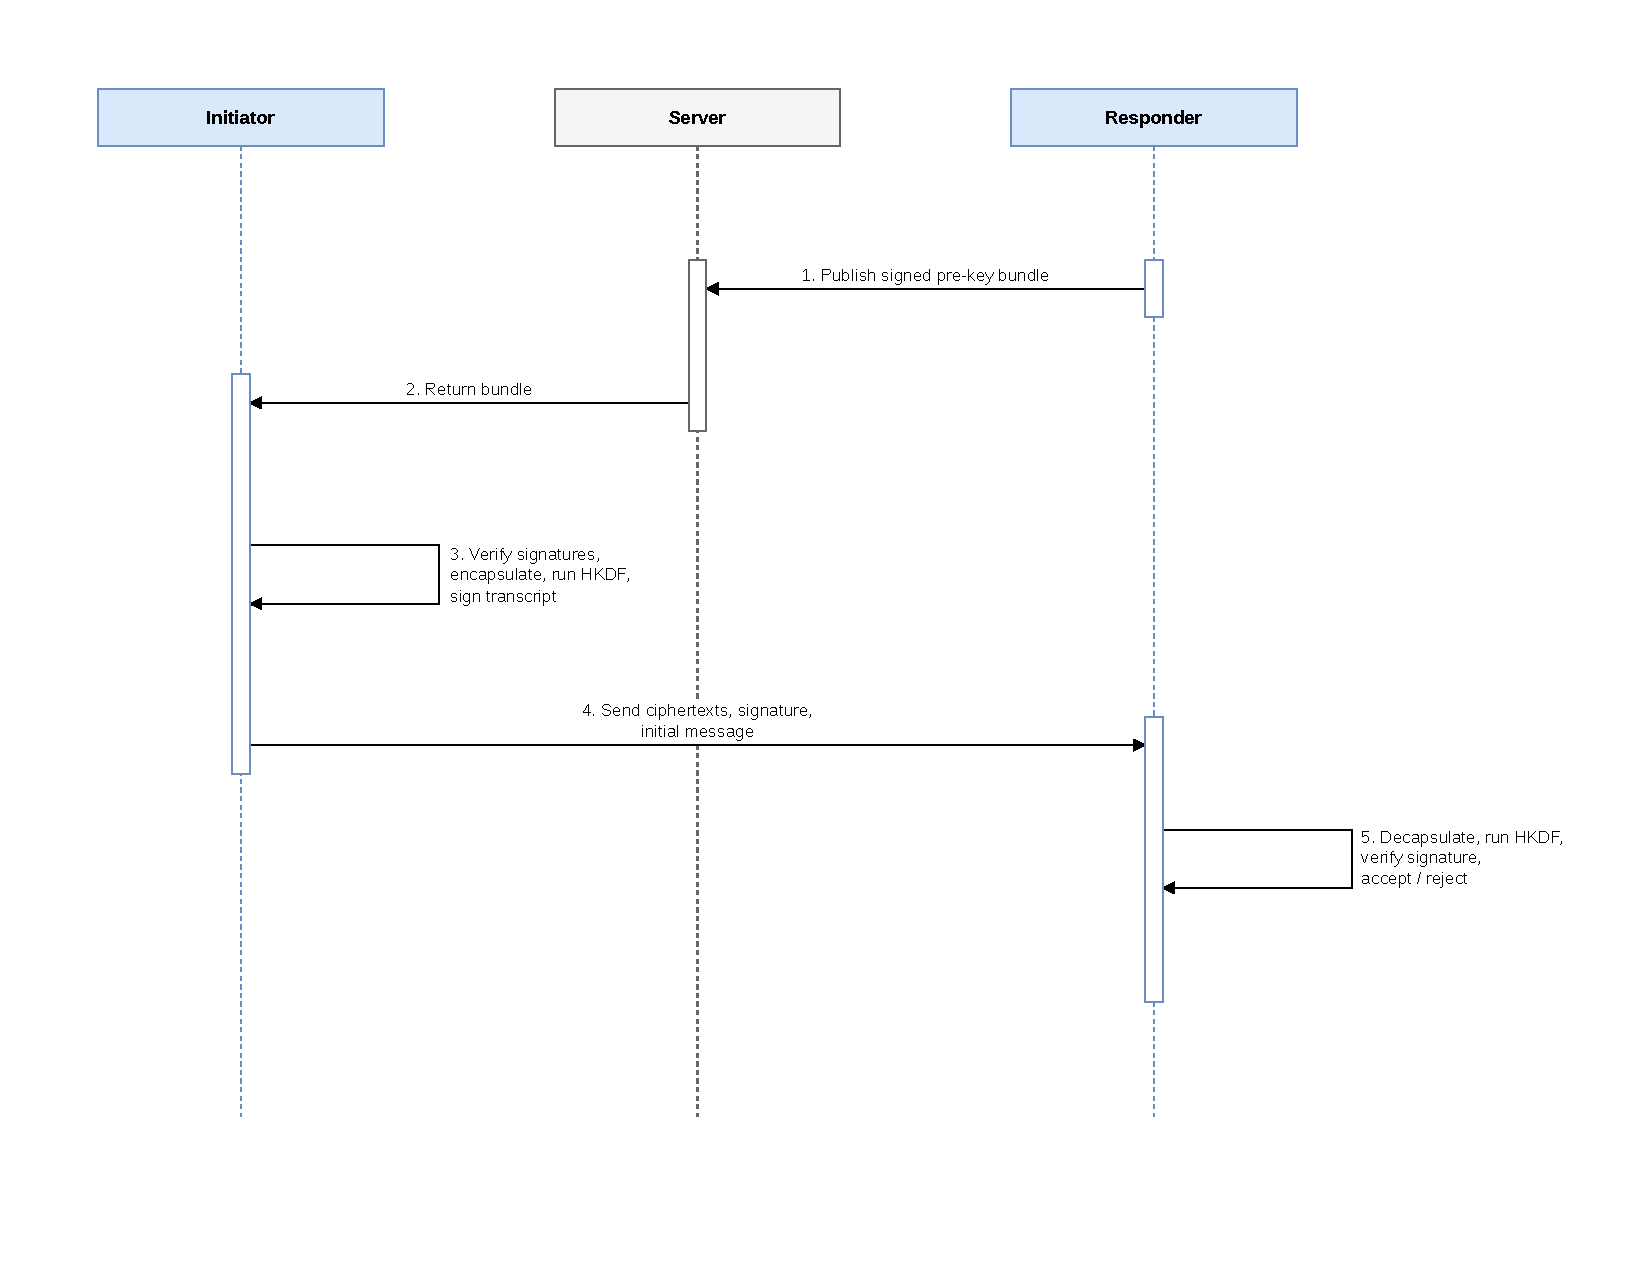
\includegraphics[width=0.95\textwidth]{assets/figures/pqxdh-derived-handshake-sequence.pdf}
    \caption{High-level message flow of the PQXDH-derived handshake shared by both source-code versions.}
    \label{fig:pqxdh-derived-handshake-sequence}
\end{figure}

Key derivation must be domain-separated by mechanism rather than solely by intent: the algorithm-suite identifier must appear in both the signed transcript and the HKDF \texttt{info} input, and all encoded key types must occupy pairwise-disjoint encoding domains. The implemented labels satisfy the first condition, naming the KEM and signature suite in both the transcript label and the \texttt{info} value, and the one-byte algorithm identifiers give encoded keys disjoint domains; domain separation complements transcript authentication and does not replace it.

The Double Ratchet then combines the KEM-derived root with an X25519 agreement before encrypting or decrypting the first payload, which is why the post-quantum claim of this chapter ends at the bootstrap and transcript-authentication boundary. Libsignal authenticates that encrypted message with an eight-byte HMAC-SHA-256 tag computed over the serialised message and both encoded identity keys, verified before AES-256-CBC decryption; the KEM ciphertext fields lie outside that encrypt-then-MAC input and rely instead on the transcript signature.

The two operational modes are last-resort-only and last-resort-plus-one-time. When the store has no one-time key, or a malicious server withholds it, the handshake falls back to the weaker profile of Section~\ref{subsubsec:req-security}, and the stronger one-time claim remains conditional while the signatures do not authenticate a key's role or identifier. Replay protection is delegated to the surrounding session state: with state retained, the Double Ratchet's message-key accounting is expected to reject the repeated payload, but no end-to-end test shows that a replayed complete initial message is rejected, and state loss or rollback can allow a last-resort-only initial message to be accepted again; replay resistance remains an unverified application-layer obligation.

Secret erasure has clear requirements but incomplete implementation evidence. Each side should erase \(ss_1\), \(ss_2\), and the assembled HKDF input immediately after derivation; the responder should delete a one-time private key after its first successful decapsulation; and the initiator should discard pending ciphertexts and the transcript signature once the responder's first reply is processed. Inspection of the pinned HQC crate shows zeroisation of selected seeds, decrypted messages, and derivation intermediates, but not of every adapter or protocol-layer copy; libsignal delegates one-time-key consumption to a store hook that the bundled in-memory store does not act on; and protocol-layer zeroisation of the shared secrets and HKDF input is not demonstrated. These are recorded as unmet requirements rather than properties of the implementation.

%Chapter 3.6
\subsection{Specification-Derived Size Comparison}
\label{subsec:theoretical-comparison}

The specifications allow the communication and storage costs to be estimated before any benchmark is run. The values in this section are lower bounds for cryptographic-component payloads, not measurements of complete serialised protocol objects or bundle-component totals; Chapter~\ref{sec:results} reports complete message-object captures, serialised bundle-component totals, and analytical storage counterparts. Keeping these quantities separate avoids presenting Protocol Buffers framing or payload-dependent encryption as if it were an intrinsic property of a KEM.

The accounting follows the artefact's encodings. Every public key and KEM ciphertext carries a one-byte algorithm identifier, while ML-DSA-87 and XEdDSA signatures carry none; an ML-DSA-87 identity verification key therefore occupies 2593 bytes, 2592 from FIPS 204 plus the \texttt{0x09} type byte. A bundle cryptographic-component sum includes the identity key, the ratchet or signed pre-key and its signature, every KEM pre-key and its signature, and the baseline's optional one-time curve key; an initial-message cryptographic-component sum includes the initiator's identity and base or ephemeral keys, the KEM ciphertext or ciphertexts, and, for Versions 1 and 2, the transcript signature. Numeric identifiers, Protocol Buffers framing, and the encrypted first message are excluded; these fields are not assumed equal between configurations, which is why Chapter~\ref{sec:methodology} measures complete initial-message and reply protocol objects separately and reports a serialised bundle-component total rather than a complete bundle encoding.

Modelled server-held public cryptographic payload is reported per device. For Versions 1 and 2 it is parameterised by \(N\), the number of stored one-time KEM pre-keys; for the baseline, the one-time KEM and curve-key inventories are represented separately by \(K\) and \(C\). A single unqualified per-user value would otherwise conceal the largest variable components. Table~\ref{tab:spec-sizes} combines the KEM and signature sizes established in Sections~\ref{subsubsec:kem-selection} and~\ref{subsubsec:sig-selection}. The baseline uses 33-byte encoded X25519 public keys and 64-byte XEdDSA signatures, and follows PQXDH's either/or selection of a one-time or last-resort Kyber pre-key \cite{kret2024pqxdh}. Its per-run KEM material is consequently one public key and one ciphertext in either mode.

\begin{table}[htbp]
    \centering
    \caption{
        Specification-derived cryptographic-component sums in bytes. Base mode denotes last-resort-only mode for the source-code versions and a baseline fetch without a one-time curve pre-key; the optional-key rows therefore compare different key roles.
    }
    \label{tab:spec-sizes}
    \begin{tabular}{lrrr}
        \hline
            Cryptographic component & Baseline & Version 1 & Version 2 \\
        \hline

            Bundle component sum, base mode & 1763 & 13449 & 19118 \\
        Bundle component sum, optional key present & 1796 & 19645 & 30983 \\
        Initial-message component sum, base mode & 1635 & 8822 & 21675 \\
        Initial-message component sum, optional key present & 1635 & 10391 & 36097 \\
        \hline
    \end{tabular}
\end{table}

The table gives three immediate results. First, the aggregate move from the baseline to Version 1 multiplies the base bundle-component sum by approximately 7.6 and the base initial-message component sum by approximately 5.4. This is not an ML-KEM overhead in isolation: it combines every protocol change listed in Section~\ref{subsubsec:kem-selection}, and the largest contribution is the ML-DSA-87 material, comprising one 2593-byte identity key and two 4627-byte signatures in the base bundle-component sum.

Second, replacing ML-KEM-1024 with HQC-256 adds 5669 bytes for each bundled KEM public key and 12853 bytes for each ciphertext. With an optional one-time KEM key, Version 2's initial-message component sum reaches 36097 bytes, approximately 22 times the baseline, isolating the principal cryptographic-payload cost of the KEM substitution more clearly than the baseline comparison does.

Third, under the public-component model, server-held payload per device is \(13449 + 6196N\) bytes for Version 1 and \(19118 + 11865N\) bytes for Version 2. The corresponding baseline is \(1763 + 33C + 1633K\) bytes, where \(C\) and \(K\) are its one-time curve- and KEM-pre-key inventories. At \(N = 100\), the two source-code versions require approximately \(633~\text{kB}\) and \(1206~\text{kB}\) per device respectively, using decimal kilobytes. The complete initial-message measurements reported in Chapter~\ref{sec:results} additionally include identifiers, Protocol Buffers field tags and length framing, and the encrypted message; bundle and server-held figures remain component-level analytical totals rather than complete service encodings.

%Chapter 3.7
\subsection{Chapter Summary}
\label{subsec:design-summary}

This chapter turned the findings of Chapter~\ref{sec:lit} into requirements, a threat model, and a selection framework; selected ML-DSA-87 for authentication and ML-KEM-1024 as the primary KEM, retaining HQC-256 as the experimental code-based comparator; and specified the two source-code versions, fixing the post-quantum claim at the bootstrap and transcript-authentication boundary. The obligations recorded along the way, role and identifier authentication, protocol-level binding, exact replay rejection, deletion of consumed one-time keys, and zeroisation, bound what the evaluation may claim: Chapter~\ref{sec:methodology} defines its measurements around these distinctions, and Chapter~\ref{sec:results} must report demonstrated, conditional, unresolved, and unmet results separately.
